\documentclass[preview]{standalone}

\usepackage{amsmath}
\usepackage{amssymb}
\usepackage{stellar}
\usepackage{tikz}
\usepackage{makecell}

\usetikzlibrary{cd}

\hypersetup{
    colorlinks=true,
    linkcolor=black,
    urlcolor=blue,
    pdftitle={Stellar},
    pdfpagemode=FullScreen,
}

\begin{document}

\title{Stellar}
\id{storia-svizzera}
\genpage

\section{Confederazione dei 13 Cantoni}

\begin{snippet}{confederazione-13-cantone-expl}
    La Confederazione dei 13 Cantoni era fondamentalmente suddivisa in 3 gruppi territoriali.
    \begin{itemize}
        \item Cantoni sovrani (13);
        \item 11 Alleati;
        \item paesi / Territori soggetti, (baliaggi).
    \end{itemize}

    Vi è una ampia autonomia delle comunità locali (Entità indipendente del Sacro Romano Impero Germanico dal 1698).
    Le città sono principalmente composte da governi oligarchici, mentre verso le comunità
    vi erano le landsgemeinde (assemblee) di contadini proprietari.
\end{snippet}

\begin{snippetdefinition}{oligarchia-definizione}{Oligarchia}
    Con \textit{oligarchia} si indica il governo di pochi (es. famiglia importanti, influenti).
\end{snippetdefinition}

\plain{La Svizzera del tempo è quindi frammentata, ma viene tenuta assieme da una Dieta.}

\begin{snippetdefinition}{dieta-svizzera-definizione}{Dieta}
    La \textit{Dieta} è un'assemblea generale di delegati dei Cantoni (e di alcuni alleati).
\end{snippetdefinition}

\begin{snippet}{0191fe2b-6263-4dc1-8312-47176f675366}
    Ogni decisione doveva essere presa all'unanimità.
    La Dieta dei cantoni cattolici si riuniva separatamente da quella di Protestanti.
    Non c'è un esercito unitario e una vera e propria politica estera.
    Inoltre, la Svizzera ha una lunga tradizione di \textit{mercenariato} che, per i cantoni più rurali,
    è un importante entrata economica.
    L'ultima Dieta avvenne nel 1798.
    A turni, ogni cantone mandava un landfogto nei comuni per essere amministratori.
    
    La Svizzera è quindi composta da enti separati che sono tutti collegati da un ente centrale, come il patto o la Dieta.
\end{snippet}

\section{Confederazione e federazione}

\begin{snippet}{federazione-vs-confederazione-svizzera}
    La confederazione è un'alleanza tra Stati, mentre la federazione è un unico Stato,
    anche se composto di parti (Stati o regioni) che godono di una larga autonomia.
    Tra una confederazione e una federazione vi sono numerose soluzioni istituzionali intermedie.
    La Svizzera è una federazione nonostante sia rimasto il nome di tradizione di confederazione.
\end{snippet}

\section{Club helvétique}

\begin{snippetdefinition}{club-helvetique-definizione}{Club helvétique}
    Il \textit{Club helvétique} è un club di svizzeri a Parigi.
    Essi comunicano con i francesi e sostengono l'espansione delle idee derivanti dalla Rivoluzione Francese
    in Svizzera.
\end{snippetdefinition}

\section{La Repubblica elvetica (1798 - 1802)}

\begin{snippet}{repubblica-elvetica-expl}
    Dal 1798 la Svizzera passa da una confederazione ad una repubblica (una e indivisibile),
    ossia un regime imposto dalla Francia.
    In questa repubblica vengono aboliti i baliaggi, ma vengono definiti come \textit{unità amministrative}.
\end{snippet}

% TODO metti le due diverse costituzioni LA SVIZZERA DALLA VECCHIA CONFEDERAZIONE AL 1848

\begin{snippet}{riforme-introdotte-dalla-repubblica-svizzera}
    Le riforme introdotte con la Repubblica sono le seguenti:
    \begin{itemize}
        \item Uguaglianza dei cittadini di fronte alla legge;
        \item suffragio universale (maschile);
        \item libertà di pensiero, di stampa, di religione;
        \item libertà di domicilio e industria;
        \item viene creata la cittadinanza svizzera: le persone non sono più unicamente cittadini dei loro cantoni;
        \item divisione dei poteri secondo il principio di Montesquieu;
        \item unificazione dei pesi, delle misure e della moneta.
        \item soppressione delle dogane interne;
        \item obbligatorietà dell'insegnamento elementare.
    \end{itemize}
\end{snippet}

\plain{La Repubblica Elvetica è tuttavia molto politicamente instabile e termina nel 1802.}

\section{Atto di Mediazione (1802/1803-1810)}

\begin{snippet}{atto-mediazione-illustration}
    \begin{center}
        \begin{tikzcd}
            & \fbox{\textit{Mediazione}} & \\
            \makecell{\text{Federalisti} \\ \text{(cattolici)}} & & \makecell{\text{Repubblicani} \\ \text{(centralisti)}}
        \end{tikzcd}
    \end{center}
\end{snippet}

\begin{snippet}{30ff5b19-7471-4919-b151-d59837fffa46}
    I federalisti sono favorevoli all'autonomia cantonale, ossia ciò che c'era prima della repubblica elvetica.
    I repubblicani sono invece favorevoli ad uno stato unitario, un unico governo indivisibile e dove i cantoni non hanno automonie.
    I federalisti sono quindi tradizionalisti, a differenza dei repubblicani.
\end{snippet}

\begin{snippetdefinition}{atto-mediazione-definizione}{Atto di mediazione}
    L'\textit{atto di mediazione} (1802/1803-1810) è stato imposto da Napoleone alla Svizzera per
    applicare una nuova Costituzione di stampo maggiormente federalistico e
    dunque con maggiori poteri attribuiti ai Cantoni.
\end{snippetdefinition}

\begin{snippet}{444820c5-2bf6-470f-a940-e32a3bf75e2d}
    Questa nuova costituzione porta alla Svizzera formata da 19 cantoni tutti di pari rango.
    La Dieta, la quale si riunisce una volta all'anno come congresso dei delegati,
    rappresenta quindi l'autorità centrale.

    I compiti e capacità della Dieta:
    \begin{itemize}
        \item promulgare dei decreti;
        \item dichiarare guerra;
        \item firmare e ratificare la pace;
        \item concludere alleanze e trattati commerciali.
    \end{itemize}

    Il potere viene suddiviso con \\
    \textbf{legislativo} \(\rightarrow\) Gran Consiglio (110 deputati) \\
    \textbf{esecutivo} \(\rightarrow\) Piccolo Consiglio.
\end{snippet}

\begin{snippet}{mediazione-illustration}
    \begin{center}
    \begin{figure}[h]
        \centering
        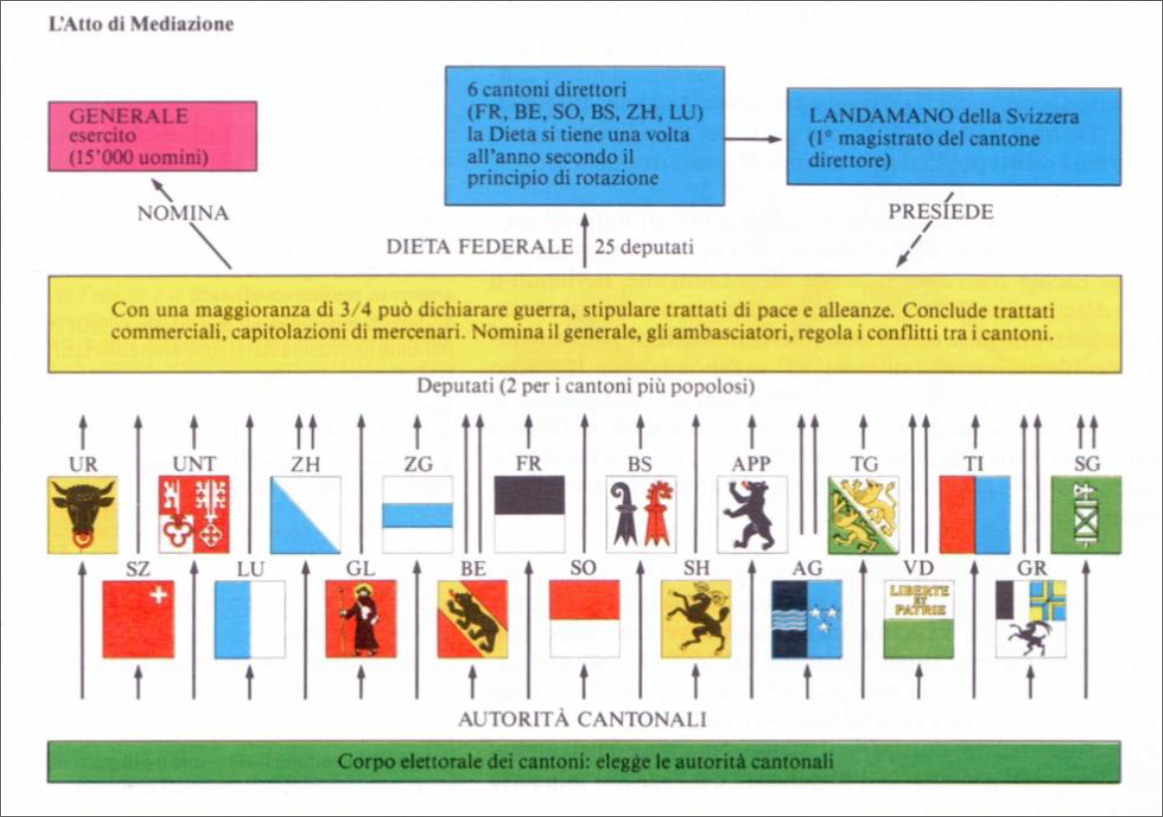
\includegraphics[width=0.75\textwidth]{./resources/mediazione.png}
    \end{figure}
    \end{center}
\end{snippet}

\section{Restaurazione}

\begin{snippet}{restaurazione-expl}
    Nel 1815 le potenze europee che avevano sconfitto Napoleone (vincitrici del Congresso di Vienna)
    volevano ripristinare in parte gli equilibri prerivoluzionari.
    In Svizzera ciò avvenne con il Patto federale del 1815 che
    accordò ai Cantoni la quasi completa autonomia amministrativa.
\end{snippet}

\begin{snippetdefinition}{patto-de-1815-definizione}{Patto del 1815}
    Il \textit{patto del 1815} è una costituzione che crea una confederazione elvetica di 23 cantoni.
\end{snippetdefinition}

\begin{snippet}{8647aae5-bd9e-4814-91ce-2575f145a2c0}
    Le potenze assicurarono alla Svizzera la neutralità perpetua e garantirono
    l'integrità e l'inviolabilità del territorio svizzero allargato.
    Esso ridisegna la cartina europea e viene riconosciuto a livello internazione la neutralità elvetica perpetua.
    \\
    La Svizzera prende il nome ufficiale di Confederazione Svizzera, con 23 cantoni sovrani.
    Nascono quindi istituzioni conservatrici in Svizzera.
    La Dieta federale esiste ancora ma ha meno potere.
    Inoltre, vi è un esercito unico per la prima volta.
    Tornano tuttavia le dogane interne, ostacolando il traffico doganale, e quindi facendo
    soffrire la Svizzera economicamente.
    La Svizzera può stipulare una pace o dichiarare una guerra se ha una maggioranza di \(\frac{3}{4}\),
    mentre per altre questioni una maggioranza semplice.
\end{snippet}

\section{Influenza liberale dal 1830}

\begin{snippet}{678af0fc-7fc7-489e-8940-2e750ff3d298}
    Nonostante la corrente restaurativa, la Svizzera rimane
    comunque aperta verso gli esuli delle altre nazioni.
    Infatti, la Svizzera diventa terra d'asilo per gli esuli del liberalismo.
    Questa situazione favorisce il progresso liberalista.
    
    Dopo la rivoluzione parigina del 1830, la metà circa dei cantoni, fra i quali Berna, Zurigo,
    Lucerna, Vaud, Friborgo riformarono le loro costituzioni in senso democratico,
    abolirono le antiche imposizioni feudali, garantirono le libertà politiche fondamentali.
    
    La riforma del sistema politico federale costituisce il principale pomo della discordia
    tra liberali-radicali e conservatori. I primi, pronti ad usare la forza per riformare il Patto
    del 1815 al fine di creare uno stato con un potere centrale più forte. I secondi, si
    pongono come i più decisi sostenitori della sovranità cantonale. Le questioni religiose
    complicano un conflitto che è essenzialmente di natura politica: i liberali radicali sono
    fautori di una società laica e vedono nel cattolicesimo un ostacolo alla modernizzazione
    del paese, che viene invece strenuamente difeso dai conservatori.
    
    In seguito ai tentativi dei radicali di rovesciare con la forza il governo di Lucerna (1844-45)
    i cantoni conservatori cattolici (Lucerna, Uri, Schwyz, Unterwald, Friburgo, Vallese)
    costituirono un'alleanza difensiva segreta, il Sonderbund (dicembre 1845), che in
    contrasto col Patto federale del 1815, prese contatto con alcune potenze straniere.
\end{snippet}

\begin{snippet}{influenza-liberale-illustration}
    \begin{center}
    \begin{tikzcd}
        \fbox{\textit{(liberali)radicali}} &  & \fbox{\textit{conservatori}} \\
        \makecell{\text{Revisione del Patto} \\ \text{del 1815}} & & \makecell{\text{Forte autonomia} \\ \text{cantonale}} \\
        \makecell{\text{Stato e società} \\ \text{laica}} & & \makecell{\text{Difesa del} \\ \text{cattolicesimo}}
    \end{tikzcd}
    \end{center}
\end{snippet}

\begin{snippetdefinition}{rigenerazione-definizione}{Rigenerazione}
    Con \textit{rigenerazione} (1831 - 1848) si intende il periodo dove una decina di Cantoni promulga nuove Costituzioni più liberali.
\end{snippetdefinition}

\begin{snippetdefinition}{Sonderbund-definizione}{Unione di difesa (Sonderbund)}
    Contro i liberali radicali alcuni Cantoni unificano un unione di difesa,
    per evitare che vi sia una rigenerazione anche nei loro Cantoni.
\end{snippetdefinition}

\begin{snippet}{e3d73132-fbf2-4b0e-9c17-db10be424a86}
    L'Unione di difesa viene tuttavia giudicata in contrasto al paragrafo 6 della Costituzione, in quanto
    viene definitiva come un'alleanza o lega separata.
    I cantoni non posso creare alleanza che possano nuocere al patto federale.
    
    Nel luglio del 1847 la Dieta si riunisce e scioglie il Sonderbund.
    I cantoni conservatori sono tuttavia in disaccordo con questa scelta e si rifiutano di scioglierla,
    nasce quindi una guerra civile.
    
    Avendo perso la guerra, una volta sciolto il Sonderbund non vi furono più ostacoli alla revisione del Patto del 1815.
    Il Sunderbund deve pagare un'indennità per aver causato la guerra.
\end{snippet}

\begin{snippetdefinition}{guerra-sonderbun-definizione}{Guerra civile del Sonderbund}
    la \textit{guerra civile del Sonderbund} (1847) è stata una guerra civile
    della durata di un mese.
\end{snippetdefinition}

\plain{Nessuna potenza straniera è intervenuta nella guerra data la sua breve durata.}

\section{Dalla Confederazione alla Federazione (1848-)}

\begin{snippet}{ee801f9c-fb46-4d55-accf-de20536e9a4c}
    Un gruppo di rappresentanti si unisce e ridige la nuova Costituzione e la presentano alla Dieta.
    Il referendum cantonale passa la decisione, e quindi tutti i Cantoni devono applicarla.
    
    Il 12 settembre 1848 la Dieta federale approva la nuova costituzione.
    Nasce quindi la Svizzera moderna, ossia uno stato federativo.
    Le questioni federali vengono quindi decise dalla maggioranza, schiacciando chi si oppone a tali decisioni.
    Queste decisioni includono quelle militari oppure circa politica estera.
    Per alcune competenze, come l'istruzione, i cantoni rimangono sovrani.
    
    La costituzione federale è direttamente ispirata a quella degli Stati Uniti.
    \begin{itemize}
        \item La sovranità su base nazionale è popolare;
        \item possono votare i cittadini sopra i 20 anni (maschi, ovviamente);
        \item i cittadini eleggono rappresentanti;
    \end{itemize}
    
    % https://tikzcd.yichuanshen.de/#N4Igdg9gJgpgziAXAbVABwnAlgFyxMJZAJgBoAGAXVJADcBDAGwFcYkQAdDgMwCMIAHsADCuHPShYwWAL4gZpdJlz5CKAIyl11Ok1bsuOGAJy9uwAIJw4MALa9GMegAIAYjFgAnJjDkKl2HgEROQUOgwsbIicHEYmwABy9ABeqj5+iiAYgaohpMThelExcTjAACIwAOaMWM4AyuJ4GQEqwShkBTQR+tGGxqbmwgTYNfhuHjDeji1ZykFqyADM+YWRBrEDZsAAKp5YvMxgPhNe6fKZ2W2LZAAsa70lA7jAAKI2AMbMeLQQs1cLIgre7dIobUovADiWGYklS9H2fwurUBGlIIN06z6mxMLwAMtUsHBGPQfkj-HMcu1kJoupjHvIdB4qvAiKBuJ4ILYkKEQDgIEhNCBeDAwFAkEteT1iv14jBHFUqgRyZkOVzBTR+UgyPSZTiymhORhPKkCL4QDQSSLGAAFea5aL7KoACxwFuFovFiElFLV3MQQq13tBWKe8WIzjQU2cH3oYH5YHNNBFYqQAFofarOf7AwLELcQ49ZWV5dUWXJLfRrXaqWoQE7XciQH6NXy8wBWZOeiVSsHY0rAUuK82+7NIADsmo7lqkxSgEGYDjYNGdTi9YGYjEYmvoWEY7EgiabLcQADYp0gCyBakfovPF453auJEgN1ud3uD2bj2PEAAOC9EAAThnW8QHvJcnzXV9N23Pld33aJDzYGRKBkIA
\end{snippet}

\section{Democrazia semidiretta}

\begin{snippet}{36835b9b-9b96-4147-95a2-af7d43c67deb}
    Si dice democrazia semidiretta perché i cittadini eleggono persone che, a loro volta,
    avranno un impatto politico.
    La sovranità popolare si applica quindi mediante rappresentanti eletti intermediari.
    
    Nel 1874 viene introdotto il \textbf{diritto di referendum facoltativo}.
    Con 30000 (50000 dal 1977) è possibile sottoporre al voto del popolo una legge già accettata dal parlamento federale.
    
    Nel 1891 viene introdotto il \textbf{diritto di iniziativa costituzionale}.
\end{snippet}

\section{I movimento politici}

\begin{snippet}{7d9a0635-80b5-44c2-8735-4ed1b58e7fce}
    \begin{itemize}
        \item Tendenza liberal-radicale: favorevole al rafforzamento dello Stato federale all'affermazione dei diritti individuali e politici.
        Nel 1894 fondano il \textbf{partito radicale - democratico}.
        Nel 2009 prende il nome di \textbf{PLR}.
        \item Tendenza conservatrice: difende l'autonomia dei cantoni e la libertà delle chiese.
        \item I cattolici-conservatori mirano alla riconciliazione tra Chiesa e Stato; nel 1894 fondano il \textbf{partito popolare cattolico}.
        Negli anni '70 diventa \textbf{PPD} e oggi \textbf{Il Centro}.
        \item Per rispondere ai problemi sociali sorti dall'industrializzazione nel 1888, nasce il \textbf{partito socialdemocratico svizzero}.
    \end{itemize}
    
    Per alcuni decenni, tutte le poltrone del governo erano in mano ai liberal-radicali (governo monopolitico).
    Nel 1891, entra per la prima volta un cattolico-conservatore (Joseph Zemp).
    Dal 1959 fino al 2003 la composizione partitica del Consiglio federale è rimasta immutata (formula magica):
    2 liberali, 2 PPD, 2 socialisti e un UDC.
\end{snippet}

\end{document}